\scanpage{170}
\diagram{\begin{tikzcd}
(z,s)\arrow[r] & (\varepsilon z\exp 2\pi as,\ \varepsilon's)
\end{tikzcd}}
\margin{$\varepsilon,\varepsilon'\in\mu$\par $a\in\unsure{\mathbb Q|\mathbf Q}$}

\figure{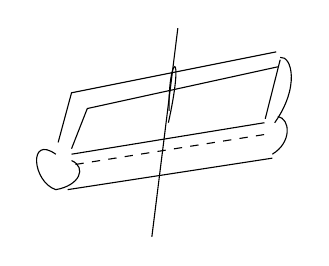
\begin{tikzpicture}[x=1cm,y=1cm]
\draw (0,.25) .. controls (-.35,.5) and (-.3,-.1) .. (0,-.2)
 .. controls (.3,-.15) and (.4,.08) .. (.2,.17);
\draw (.15,-.2)--(2.75,.2);
\draw (.2,.25)--(2.65,.65);
\draw[dashed] (.25,.12)--(2.65,.5);
\draw (.03,.4)--(.2,1.03)--(2.8,1.55);
\draw (.2,.32)--(.4,.83)--(2.82,1.36);
\draw (2.75,.25) .. controls (3,.4) and (2.98,.7) .. (2.82,.73);
\draw (2.78,.65)..controls (3.1,1.1) and (3,1.5)..(2.85,1.48);
\draw (2.66,.7)--(2.85,1.45);
\draw (1.22,-.8)--(1.55,1.85);
\draw (1.43,.65)..controls (1.65,1.65) and (1.42,1.5)..(1.44,.8);
\end{tikzpicture}}
\[
(z\exp 2i\pi as)^{(-1)^\nu},\quad\varepsilon s
\]
\[
\deleted{\varepsilon\ \varepsilon'}\qquad D_\infty\times\mu
\]
\figure{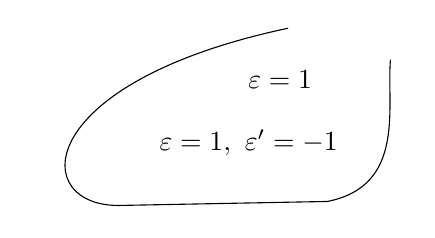
\begin{tikzpicture}
\draw (2.3,1.8)..controls (-1,1.1) and (-1,-.5)..(.2,-.45)
 --(2.8,-.4)..controls (3.8,-.2) and (3.55,.8)..(3.6,1.4);
\node at (2.2,1.15) {$\varepsilon=1$};
\node at (1.8,.35) {$\varepsilon=1,\ \varepsilon'=-1$};
\end{tikzpicture}}

\figure{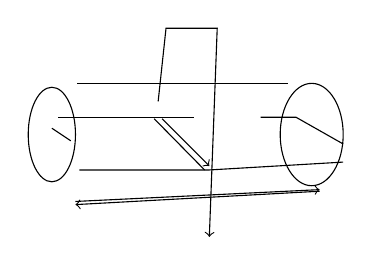
\begin{tikzpicture}[x=1cm,y=1cm]
\draw (0,0) ellipse (.3 and .6);
\draw (3.3,0) ellipse (.4 and .65);
\draw (.32,.65)--(3,.65);
\draw (.35,-.45)--(2,-.45)--(3.7,-.35);
\draw (.08,.22)--(1.8,.22);
\draw (2.65,.22)--(3.1,.22)--(3.7,-.12);
\draw (0,.08)--(.24,-.08);
\draw[->] (1.35,.42)--(1.45,1.35)--(2.1,1.35)--(2,-1.3);
\draw[->] (1.4,.2)--(2,-.4);
\draw (1.3,.2)--(1.94,-.45);
\draw[->] (.3,-.85)--(3.4,-.7);
\draw[->] (3.4,-.72)--(.3,-.89);
\end{tikzpicture}}
\[
\sigma_1(z,s)=(z^{-1},s)\qquad
\underline a(z,s)=(-z,-s)
\]
\[
\sigma_2(z,s)=(z,\deleted{\unsure{-}}s)
\]
\[
\deleted{\unsure{\rho}}\Theta(z,s)=(z\exp 2i\pi s,s)
\]
\figure{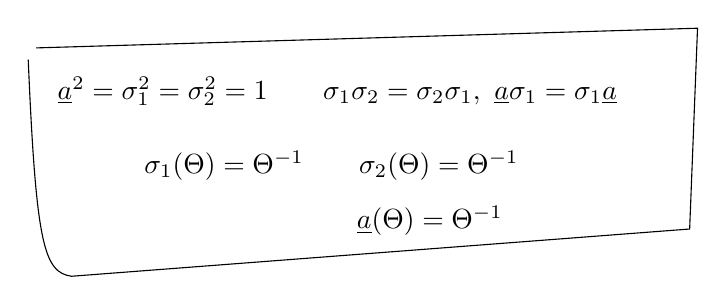
\begin{tikzpicture}[x=1cm,y=1cm]
\draw (0,2.1)--(8.4,2.35)--(8.3,-.2)--(.45,-.8)
 .. controls (.1,-.75) and (0,-.4)..(-.1,1.95);
\node[anchor=west] at (.15,1.55)
 {$\underline a^2=\sigma_1^2=\sigma_2^2=1\qquad
 \sigma_1\sigma_2=\sigma_2\sigma_1,\ 
 \underline a\sigma_1=\sigma_1\underline a$};
\node[anchor=west] at (1.25,.6)
 {$\sigma_1(\Theta)=\Theta^{-1}\qquad\sigma_2(\Theta)=\Theta^{-1}$};
\node at (5,-.1) {$\underline a(\Theta)=\Theta^{-1}$};
\end{tikzpicture}}
\margin{\[
\begin{gathered}
(z^{-1}\exp 2i\pi s,s)\\
(z\exp -2i\pi s,s)\unsure{)}\\
z\exp -2i\pi s,+s\\
-z\exp -2i\pi s,-s\\
z\exp -2i\pi s,s)
\end{gathered}
\]}
\[
\underline a\quad\alpha,\beta,\Theta
\]
\margin{170}
